\documentclass[11pt]{article}
\usepackage[margin=1in]{geometry}
\usepackage{amsmath, amssymb}
\usepackage{enumitem}
\usepackage{tikz}
\usepackage{tikz-qtree}
\usetikzlibrary{arrows.meta, positioning, graphs, automata, matrix, calc}

\setlength{\parindent}{0pt}
\setlength{\parskip}{0.5em}
\setlist{nosep}

\tikzset{
    every tree node/.style={circle, draw, minimum size=0.6cm, inner sep=1pt},
    blank/.style={draw=none, fill=none, edge from parent/.style={draw=none}},
    blacknode/.style={circle, draw, fill=black, text=white, minimum size=0.6cm, inner sep=1pt},
    whitenode/.style={circle, draw, fill=white, text=black, minimum size=0.6cm, inner sep=1pt},
    rednode/.style={circle, draw, fill=white, text=black, minimum size=0.6cm, inner sep=1pt},
    tfnode/.style={rectangle, draw, rounded corners=2pt, minimum size=0.45cm, inner sep=1pt},
    listnode/.style={rectangle, draw, rounded corners=2pt, minimum height=0.6cm, inner sep=3pt},
    skipnode/.style={rectangle, draw, minimum size=0.6cm, inner sep=2pt},
    main node/.style={circle, draw, minimum size=0.6cm}
}
\begin{document}

\begin{center}
    \Large\textbf{CS 253: Data Structures and Algorithms}\\
    \large\textbf{Randomized Final Study Problem}
\end{center}
\vspace{1em}

% seed=1
% topic=ford_fulkerson
% vertices=6
% edges=12
% augmentations=4
% max_flow=15

\section*{Graphs}
\subsection*{Ford-Fulkerson Maximum Flow}
Starting with an initial flow of 0 on every edge, perform the Ford-Fulkerson algorithm to find the maximum flow from $s$ to $t$. For each iteration, show the augmenting path, its bottleneck capacity, and the updated flow values.

\begin{center}
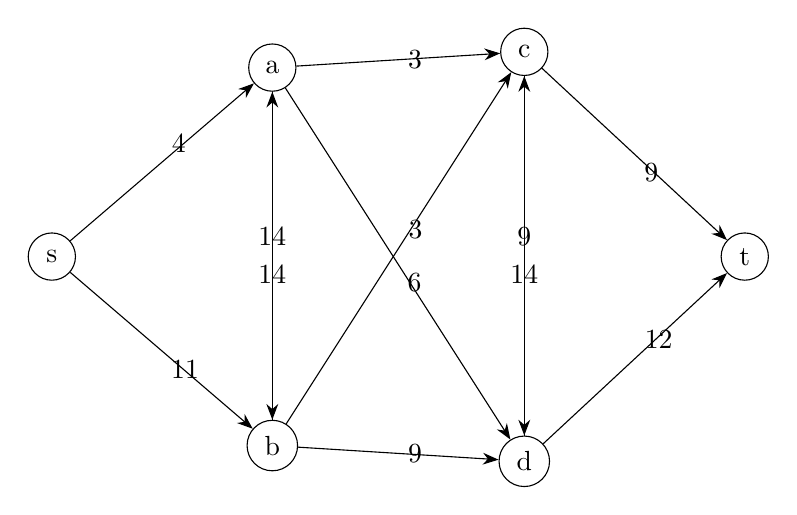
\begin{tikzpicture}[>={Stealth[length=2mm]}, main node/.style={circle,draw,minimum size=0.6cm}]
% Flow network with capacities for Ford-Fulkerson tracing.
  \node[main node] (0) at (0.0, 0.0) {s};
  \node[main node] (1) at (2.8, 2.4) {a};
  \node[main node] (2) at (2.8, -2.4) {b};
  \node[main node] (3) at (6.0, 2.6) {c};
  \node[main node] (4) at (6.0, -2.6) {d};
  \node[main node] (5) at (8.8, 0.0) {t};
  \draw[->] (0) edge node[above right] {4} (1);
  \draw[->] (0) edge node[below right] {11} (2);
  \draw[->] (1) edge node[below] {14} (2);
  \draw[->] (2) edge node[above] {14} (1);
  \draw[->] (1) edge node[right] {3} (3);
  \draw[->] (1) edge node[below right] {6} (4);
  \draw[->] (2) edge node[above right] {3} (3);
  \draw[->] (2) edge node[right] {9} (4);
  \draw[->] (3) edge node[below] {14} (4);
  \draw[->] (4) edge node[above] {9} (3);
  \draw[->] (3) edge node[below right] {9} (5);
  \draw[->] (4) edge node[above right] {12} (5);
\end{tikzpicture}
\end{center}

\subsection*{Instructor Reference}
Maximum flow value: 15.
Augmenting path sequence: s$\to$a$\to$c$\to$t (bottleneck 3); s$\to$a$\to$d$\to$t (bottleneck 1); s$\to$b$\to$c$\to$t (bottleneck 3); s$\to$b$\to$d$\to$t (bottleneck 8).
Final edge flows (flow/capacity): s$\to$a:4/4, s$\to$b:11/11, a$\to$b:0/14, b$\to$a:0/14, a$\to$c:3/3, a$\to$d:1/6, b$\to$c:3/3, b$\to$d:8/9, c$\to$d:0/14, d$\to$c:0/9, c$\to$t:6/9, d$\to$t:9/12.

\end{document}
